\documentclass{standalone}
\usepackage{pgfplots}

\pgfplotsset{compat=1.16,width=16cm}

\begin{document}
	
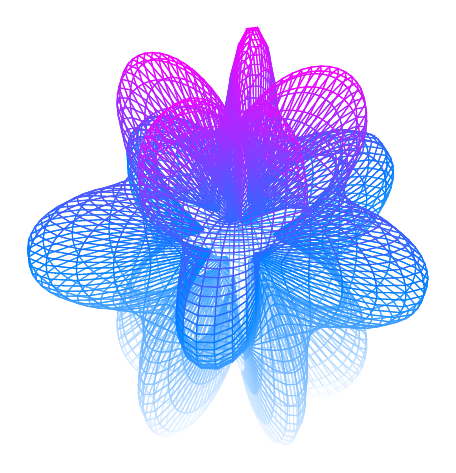
\begin{tikzpicture}
	\begin{axis}[
		hide axis,
		axis equal image,
		view={135}{30}, % Adjust the view angle for better 3D visualization
		colormap/cool,
		]
		% Plot the sphere with fluctuating waves
		\addplot3[
		thin,
		mesh,
		samples=75, % Higher samples for smooth waves
		domain=0:360,
		y domain=0:180,
		] 
		(
		{ (1 + 0.7*sin(3*y) * cos(5*x)) * sin(y) * cos(x) }, % x with wave fluctuation
		{ (1 + 0.7*sin(3*y) * cos(5*x)) * sin(y) * sin(x) }, % y with wave fluctuation
		{ (1 + 0.7*sin(3*y) * cos(5*x)) * cos(y) }           % z with wave fluctuation
		);
	\end{axis}
\end{tikzpicture}
	
\end{document}
